\PassOptionsToPackage{utf8}{inputenc}
\documentclass{bioinfo}

\usepackage[draft]{hyperref}

\newcommand{\vocab}{\textbf}

\copyrightyear{XXXX} \pubyear{XXXX}

\access{Advance Access Publication Date: Day Month Year}
\appnotes{Genome Analysis}

\begin{document}
\firstpage{1}

\subtitle{Genome Analysis}

\title[short Title]{Efficient dynamic variation graphs}
\author[Eizenga, \textit{et~al}.]{
Jordan M. Eizenga\,$^{\text{\sfb 1, \sfb 2} \dagger}$, 
Adam M. Novak\,$^{\text{\sfb 1, \sfb 2} \dagger}$, 
Emily Kobayashi\,$^{\text{\sfb 1, \sfb 3}}$,
Flavia Villani\,$^{\text{\sfb 4, \sfb 5}}$,
Cecilia Cisar\,$^{\text{\sfb 1, \sfb 2}}$,
Simon Heumos\,$^{\text{\sfb 6}}$,
Glenn Hickey\,$^{\text{\sfb 1}}$,
Vincenza Colonna\,$^{\text{\sfb 4}}$,
Benedict Paten\,$^{\text{\sfb 1, \sfb 2}}$,
and Erik Garrison\,$^{\text{\sfb 1, \sfb 2}*}$
}

\address{
$^{\text{\sf 1}}$Genomics Institute, University of California Santa Cruz, Santa Cruz, CA, USA, 95064, and \\
$^{\text{\sf 2}}$Biomolecular Engineering and Bioinformatics, University of California Santa Cruz, Santa Cruz, CA, USA, 95064, \\
$^{\text{\sf 3}}$Bioinformatics and Systems Biology, University of California San Diego, La Jolla, CA, USA, 92093, \\
$^{\text{\sf 4}}$Institute of Genetics and Biophysics, Consiglio Nazionale di Ricerche, Naples, Italy, 80131, \\
$^{\text{\sf 5}}$Biotecnologie Mediche, Universit\`a degli Studi di Napoli Federico II, Naples, Italy, 80138, and \\
$^{\text{\sf 6}}$Quantitative Biology Center (QBiC), University of T\"ubingen, T\"ubingen, Germany, 72076
}

\corresp{$^\ast$To whom correspondence should be addressed. \\
$^\dagger$Contributed equally.}

\history{Received on XXXXX; revised on XXXXX; accepted on XXXXX}

\editor{Associate Editor: XXXXXXX}

\abstract{
\textbf{Motivation:} Pangenomics is a growing field within computational genomics.
Many pangenomic analyses use bidirected sequence graphs as their core data model.
However, implementing and correctly using this data model can be difficult, and the scale of pangenomic data sets can be challenging to work at.
These challenges have impeded progress in this field.\\
\textbf{Results:} Here we present a stack of two C++ libraries, \texttt{libbdsg} and \texttt{libhandlegraph}, which use a simple, field-proven interface, designed to expose elementary features of these graphs while preventing common graph manipulation mistakes.
The libraries also provide a Python binding.
Using a diverse collection of pangenome graphs, we demonstrate that these tools allow for efficient construction and manipulation of large genome graphs with dense variation.
For instance, the speed and memory usage is up to an order of magnitude better than the prior graph implementation in the \textsc{vg} toolkit, which has now transitioned to using \texttt{libbdsg}'s implementations.\\
\textbf{Availability:} \texttt{libhandlegraph} and \texttt{libbdsg} are available under an MIT License from \url{https://github.com/vgteam/libhandlegraph} and \url{https://github.com/vgteam/libbdsg}. \\
\textbf{Contact:} \href{erik.garrison@ucsc.edu}{erik.garrison@ucsc.edu} \\
\textbf{Supplementary information:} Supplementary data are available at \textit{Bioinformatics} online.
}

\maketitle

\section{Introduction}

As increasingly many individuals have been sequenced from certain species, the field of \vocab{computational pangenomics} has emerged to analyze whole populations of genomes rather than individual genomes \citep{computational2016computational}.
Much of the research in computational pangenomics has coalesced around graph-based approaches for representing populations of genomes \citep{Paten_2017}.
Unlike conventional string-based representations, graph data structures can represent genomic variation like substitutions, insertions, deletions, and other more complex genomic events.

Graph-based data structures present new computational challenges.
In addition to sequence, genome graphs must represent topology.
Given the size of many genomes, this can be quite demanding on computer memory.
However, the total information content in a genome graph is only incrementally more than the sequences of the pangenome.
This suggests that significant memory savings should be possible.
There is also significant impetus to make the graph data structures computationally efficient, since they are frequently the core data structure in pangenomics applications.

Early versions variation graph toolkit (\textsc{vg}) \citep{Garrison_2018} have provided a cautionary tale of a na\"ive implementation.
\textsc{vg} used full-width machine words as identifiers for graph elements and stored the elements and graph topology in a set of hash tables.
Loading the 1000 Genomes Project's variant set into the \textsc{vg} toolkit used to consume more than 300~GB of memory, which is $\sim$30 times as large as the serialized representation \citep{Garrison_2019}.

Although \textsc{vg} provided a memory-efficient representation of the graph (\textsc{xg}) that could be used during read mapping and variant calling, this representation did not allow for dynamic updates to the graph.
The dynamic implementation remained necessary for graph-modifying steps of \textsc{vg} pipelines, such as the original construction of the graph and augmenting the graph with novel variants.
Some pipelines could be made feasible by breaking large graphs into connected components.
However, this strategy reduces efficiency, and it is untenable for pangenome graphs that consist of a single component.

To overcome this limitation, we have developed three new graph genome data structures that are both dynamic, in that they allow efficient updates and edits, \emph{and} memory-efficient for real world genome graphs.
Here, we compare the performance of these data structures to those originally in \textsc{vg} as well as \textsc{xg} using a diverse collection of genome graphs obtained during our work in graphical pangenomics.

In addition to demonstrating the possibility of working with large, complex graphs in small amounts of memory, these implementations expose a common API based on the \textsc{HandleGraph} model described below.
This model provides an interface to genome graphs, based on their fundamental elements, which is intended to be implementable atop a broad diversity of graph storage designs.
The \textsc{vg} toolkit has been refactored to use this API as its default means of serializing and manipulating graphs since version 1.22.0. 

%To support reuse by other researchers,
We have packaged these implementations behind equivalent C++ and Python APIs in \texttt{libbdsg}.
This software library will reduce the need for individual research groups to continually reimplement these core data structures and ease the development of algorithms that manipulate large, complex pangenome graphs.
Moreover, the reduction in memory requirements makes it possible to move workloads that would otherwise need specialized high-memory machines onto cheaper ones that often also have more processing power (for example, from Amazon's r4 instances to c5 instances).
Combined with improvements in access speed over the previous \textsc{vg} dynamic graph implementation, significant cost and time savings can be realized.

\begin{methods}

\section{Implementation}

\subsection{Data model}

Our libraries adopt node-labeled bidirected graphs as a formalism for sequence graphs.
In a bidirected graph, nodes are considered to have left and right ``sides'', and edges connect two sides rather than two nodes.
In bidirected sequence graphs, a node's sides correspond to the 5' and 3' ends of its DNA sequence. 
Nodes can be traversed either from left to right, which is interpreted as the forward strand of the sequence, or from right to left, which is interpreted as the reverse complement.
This provides a natural means to encode DNA strandedness.

Longer sequences can be formed by concatenating the sequences of multiple adjacent nodes together.
These nodes form a path, which is defined as a list of oriented nodes (either forward or reverse), such that the graph contains an edge between the adjacent sides of each pair of subsequent oriented nodes in the list\footnote{Unlike the usage in many graph theoretic contexts, we do not intend the term path to indicate that these nodes must be distinct.}.
Some paths correspond to sequences of interest, such as reference genomes or annotations of the reference.
Because paths like these are so frequently important in practice, our graph formalism also includes a set of paths along with the graph's node and edges.

\subsection{The \textsc{HandleGraph} interface}

The \texttt{libhandlegraph} library describes an interface that exposes basic operations on our sequence graph data model.
The \textsc{HandleGraph} model focuses on five fundamental entities in bidirected sequence graphs (Figure \ref{fig:graph}):

\begin{itemize}
\item \emph{Nodes} identify pairs of complementary DNA strands and have unique numerical identifiers (IDs).
\item \emph{Strands} identify one strand of a node's DNA sequence.
\item \emph{Edges} link pairs of strands, in order.
\item \emph{Paths} represent sequences of interest as paths through the graph.
\item \emph{Steps} describe paths' visits to nodes' strands.
\end{itemize}

The defining feature of the model is that none of these entities are accessed directly.
Instead, they are accessed via \emph{handles}, which are references modeled after the concept of file handles.
The handles are implemented as a data type with no methods and no prespecified meaning for its contents.
Thus, we say that handles are ``opaque'' in that user code cannot usefully look inside them or manipulate their contents.
Rather, the \texttt{libhandlegraph} interface requires the sequence graph implementation to be able to provide or consume these handles for all queries.

%The handles are then passed back to the API to refer to these entities when performing operations and making queries.
For example, we could obtain a handle to a strand from a \textsc{HandleGraph} implementation by providing the node's ID.
We could then provide this handle to another of the graph's methods to obtain handles to this strand's neighbors, and a further method would map the neighbors' handles to their node IDs.
Alternatively, we could obtain a handle to a path from its name (e.g. ``chr22''), and then iterate over handles to the path's steps to follow its course through the graph.
%The actual contents of a handle are unspecified, which gives significant flexibility to the implementation.
%An implementation need not actually store the handle in its unpacked form.
%Handles might be implicitly represented internally, in minimal space.

One benefit of this design is that any algorithm designed for one \textsc{HandleGraph} implementation can be applied to all other implementations.
Since the actual contents of a handle are unspecified, this benefit is achieved while simultaneously maintaining flexibility in the implementation.
Another benefit is that, since the user works only through handles that they cannot forge or modify, their ability to make mistakes can be restricted.
For example, the interface can enforce the constraints on paths through bidirected graphs during edge traversal.
Furthermore, implementations can be made memory-safe by eliminating raw pointers and other direct access to graph elements.

%This prevents common mistakes that the developers identified in their work on the VG project.
%Taken together, these benefits enable code that focuses on the algorithms rather than on boilerplate bookkeeping.

\begin{figure}
	\begin{center}
		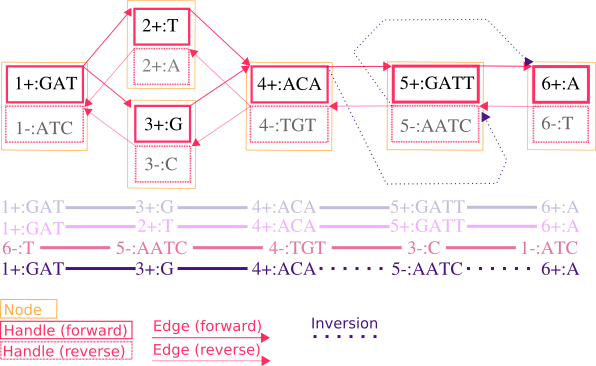
\includegraphics[width=0.5\textwidth]{figures/GRaphchrXpaper.png}
	\end{center}
	\caption{{\label{fig:graph}
        \textbf{Entities in the bidirected sequence graph.}
        Top: a variation graph showing \emph{nodes} (yellow rectangles), each of which contain a forward and reverse \emph{strand} (red solid and dashed rectangles, respectively).
        Strands show the node identifier, the direction ($+$ or $-$), and the sequence of the strand.
        Note that reverse strands show the reverse complement sequence of the forward strand.
        All \emph{edges} are shown as connections between nodes, with forward-to-forward edges denoted by solid lines, while reverse-to-reverse edges denoted by dotted lines.
        Two edges that invert from forward to reverse and reverse to forward are shown with dotted lines.
        Edges run from the strand at their beginning to their end, as indicated by the arrowhead.
        Bottom: an illustration of four \emph{paths}.
        (Each has an implicit handle, and a name, which are omitted for brevity.)
        Each path is shown in its natural direction as a series of connected \emph{steps} that refer to strands in the graph.
        The first two paths differ by a SNP, with one passing through \texttt{2+:T}, and the other through \texttt{3+:G}.
        The third path is the reverse complement of the first.
        The fourth is the same as the first, but contains an inversion, passing through \texttt{5-:AATC} rather than \texttt{5+:GATT}.
      }
    }
\end{figure}

\subsection{Graph implementations}

We consider five implementations of the \textsc{HandleGraph} model.
To ground our experimental results, here we we provide a high-level overview of each implementation.
Two implementations, \textsc{vg} and \textsc{xg}, have been described previously \citep{Garrison_2018,Garrison_2019}.
The others are combined in the \texttt{libbdsg} library (\url{https://github.com/vgteam/libbdsg}), which provides three concrete implementations: \textsc{HashGraph}, \textsc{odgi}, and \textsc{PackedGraph}.
Each implementation represents a different tradeoff in terms of speed, memory use, and capabilities.
All of the implementations except \textsc{xg} are dynamic.
They support efficient addition and deletion of nodes, edges, paths, and steps, as well as some specialized methods such as splitting a node into multiple shorter nodes.
Since all of these implementations use the same interface, the \texttt{libhandlegraph} header files serve as the most effective developer documentation for their functionality.
%Readers seeking a precise description of each implementation should refer to developer documentation and code referenced in this section.

\subsubsection{\textsc{vg}}

We have extended the data model in \textsc{vg}, previously described in \citep{Garrison_2018}, to match the \textsc{HandleGraph} API.
The backing data structures used by the model remain the same.
The graph entities are stored as objects in a backing vector, and referred to internally by hash tables that map between node identifiers and pointers into this vector.
Edges are indexed in a hash table mapping pairs of handles to edge objects.
Paths are stored in a set of linked lists, with a hash table mapping between nodes and path steps.
This arrangement was tenable for the early development of algorithms working on variation graphs.
Its inefficiency, caused by unnecessary overheads and data duplication, has generated significant difficulty for groups working with \textsc{vg}.
The other \textsc{HandleGraph} implementations respond to the limitations of this approach.
In version 1.22.0, vg was updated to use \textsc{HashGraph} (below) as the default format, though it remains compatible with all implementations described in this paper via the \textsc{HandleGraph} API.

%Its documentation can be found at \url{https://vgteam.github.io/vg/classvg_1_1VG.html}.

\subsubsection{\textsc{xg}}

\textsc{xg} was initially developed in response to the memory and runtime costs of \textsc{vg}, which prevent its application to large graphs.
It additionally provides positional indexes over paths that are required for read mapping and variant calling, and is the graph data model used in most established bioinformatic operations on variation graphs \citep{Garrison_2018,hickey2020genotyping}.
Unlike other \textsc{HandleGraph} implementations, \textsc{xg} is a static graph index.
This permits a more powerful set of efficient queries against the graph, especially for paths.
The encoding is designed to balance speed and low memory usage.
The topology of the graph is encoded in a single vector of bit-compressed integers, which promotes cache efficiency.
Rank and select operations on succinct bit vectors are used to provide random access over the variable-length records, which each encode a node's sequence, ID, and edges.
Embedded paths are encoded in variable-length integer vectors with Elias gamma encoding.
Rank and select operations on succinct bit vectors also provide queries by base-pair position along paths.
%Its documentation can be found at \url{https://github.com/vgteam/xg/blob/master/README.md}.

\subsubsection{\textsc{HashGraph}}

\textsc{HashGraph} is a relatively simple encoding, which is largely similar to the original \textsc{vg} graph.
As such, it can be seen as a streamlined point of comparison for the other new dynamic graph implementations.
However, the simplicity of this encoding has the benefit of allowing fast queries.
Thus, even though \textsc{HashGraph} still has relatively high memory requirements, it can still be useful in high memory compute environments or for small sequence graphs (such as subgraphs of genome graphs).

Like \textsc{vg}, \textsc{HashGraph} encodes the topology of the graph in a hash table indexed by node IDs.
However, these hash tables have been consolidated to avoid storing the keys multiple times.
The hash table it uses is a drop-in replacement for the equivalent standard library (STL) data structure that has been shown to outperform it in empirical evaluations \citep{brehm2019hash}.
Each hash table entry contains the sequence, an adjacency list of the edges in two STL vectors, and a vector indicating the path steps that the node can be found on.
The graph's paths are represented using doubly-linked lists to support efficient modification at any position.

In contrast to the more memory-efficient implementations, all of these data structures support computation in their native in-memory representation.
Thus, the run time to access graph elements does not also include decompressing the data.
This is how \textsc{HashGraph} maintains its comparative speed advantage.

%\textsc{HashGraph} has speed and simplicity as its primary goal.
%The data structures used in HashGraph are largely similar to the original \textsc{vg} graph.
%It represents the graph nodes as a collection of node objects in a \texttt{sparsepp} hash table (selected due to our familiarity with the project and its ability to outperform the standard library \citep{brehm2019hash}), while paths are implemented as doubly-linked lists.
%Edges are recorded in vectors attached to each node that they connect.
%This adjacency list encoding is appropriate for genome graphs, which are typically very sparse.
%Each node object maintains a vector of pointers to the path steps that traverse it.
%Most of \textsc{HashGraph}'s component data structures are uncompressed STL objects which can be used efficiently in their native in-memory arrangement.
%\textsc{HashGraph} trades memory for time, and thus is most appropriate for small graphs (from small genomes or small regions of larger genomes) or for high-memory compute environments.
%Its implementation can be found at \url{https://github.com/vgteam/libbdsg/blob/master/include/hash_graph.hpp}.

\subsubsection{\textsc{odgi}}

\textsc{odgi} (Optimized Dynamic Graph Implementation) is based on a node-centric encoding of the graph that is designed to improve cache efficiency when traversing or modifying the graph.
This encoding is split between graph topology and paths, which is important for achieving a balance of runtime performance and memory usage on graphs with large path sets.
Each node $\mathcal{N} = ( \mathcal{B}, \mathcal{P} )$ is represented by a structure that contains a byte array $\mathcal{B} = (\mathcal{Q}, \mathcal{E})$ encoding its sequence and associated edges, and a compressed integer vector $\mathcal{P} = \mathcal{S}_1 \ldots \mathcal{S}_{s}$ describing the path steps that traverse it.
The full graph model is simply an array of these node records $\mathcal{G} = \mathcal{N}_1 \ldots \mathcal{N}_{|\mathcal{G}|}$ with some additional data structures to allow for random access of paths by name, and to maintain important statistics about the size of the graph and its path set.
\textsc{odgi} uses delta encoding of edges and path steps to reduce the cost of representing graphs with local partial order and sparsity, both of which are common features of pangenome graphs.

Each node's sequence $\mathcal{Q}$ is stored using a full byte per character at the start of the byte array $\mathcal{B}$.
This allows the application of the method to protein as well as DNA sequence graphs, and allows for copy-free reference to the node sequences which can improve the performance of algorithms which interact with the sequence space of the graph.
The edges that begin or end at the node are recorded in the remainder of $\mathcal{B}$, encoded as deltas between the rank of the other end of the edge and the current node. 

%The set of $s$ steps traversing the node is recorded as an array of step records $\mathcal{P} = \mathcal{S}_1 \ldots \mathcal{S}_{s}$.
The path steps are recorded as a series of records in a dynamic integer vector which is compressed so that only the largest integer entry is stored at full bit-width \citep{prezza2017framework}.
Each step $\mathcal{S} = (p_{id}, \delta_p, \delta_n, r_p, r_n)$ contains a path identifier $p_{id}$, references to the previous $\delta_p$ and next $\delta_n$ node ID and strand on the path encoded as deltas relative to the current node, and the ranks of the previous and next steps among the path steps on their respective nodes, $r_p$ and $r_n$.
This path encoding scheme is similar to that used in the dynamic GBWT \citep{Siren_2019}, but differs in that the paths are not prefix-sorted.
%It is designed to exploit the sparse and orderable nature of genome graphs.
%If the graph is topologically sorted and node identifiers reflect this sort, the each path step will tend to connect nodes which have a small difference in identifier space.
Each path is thus conceptually a bidirectional linked list that allows efficient insertions, deletions, and replacements of path steps, encoded in a manner that exploits common properties of pangenome graphs.
%(e.g. from $n_{5} \to n_{7}$), then the maximum bit-width of the path vector will be low, resulting in good compression.

\subsubsection{\textsc{PackedGraph}}

\textsc{PackedGraph} is designed to have a very low memory footprint.
The backing data structures are implemented using bit-compressed integer vectors.
The bit-width of these vectors is chosen dynamically, starting with a bit-width of 1 and  then reallocating the vector at a higher width whenever an edit operation introduces an integer that is too large to be represented with the current width.
In the typical case that the value of $i$-th entry in the vector is $O(i)$, these reallocations have an  $O(1)$ amortized run time per edit.

Many of the integer vectors tend to also have entries that are highly correlated with their neighbors.
\textsc{PackedGraph} exploits this characteristic to achieves greater compression by only storing one entry per fixed-size window at full bit-width.
 The rest of the entries are stored in a separate integer vector and expressed as a difference from that entry.
 Since the differences within a window tend to be small, this encoding keeps the bit-width for each window small as well.

The data associated with each node is recorded in several compressed integer vectors (at the same index in each).
This contrasts to \textsc{xg} and \textsc{odgi}, which encode data in a single vector to improve cache efficiency.
Recording only one homogenous data type in a vector increases the correlation between neighboring values, which in turn improves compression.
The adjacency list for the graph, the steps that each node is found on, and the paths themselves are represented using linked lists.
The linked lists are expressed using the same bit-compressed integer vectors, where pointers are created by treating some integer entries as indexes into the vector itself.
This pointer encoding also guarantees the technical condition that the $i$-th entry is $O(i)$.
The linked lists that occur on every node (the adjacency lists and node step lists) are included in a single vector across all nodes.
This serves two purposes.
First, the windowed compression scheme in the integer vectors is inefficient if lists are smaller than the window size, as is often the case.
Second, due to the local partial order that is found in many pangenome graphs, neighboring nodes often connect to the same nodes and are found on the same paths as each other, so the values they store are also highly correlated.
%Most of its component data structures are---conceptually speaking---linked lists.
%However, they are implemented using vectors of bit-compressed integers, where pointers are produced by treating some of the integer entries as indexes into the vector that contains them.
%The bit-width can be determined dynamically.
%Doing so does not affect the amortized asymptotic run time of graph operations in the typical case that the value of $i$-th entry in the vector is $O(i)$.
%The vector uses a windowed bit compression scheme in which only one value within a window is maintained at its full bit-width.
%The remaining entries are represented as differences from this value.
%In the typical case where adjacent entries in the vector are highly correlated, this helps keep the bit-width low and the compression high.
%Its implementation can be found at \url{https://github.com/vgteam/libbdsg/blob/master/src/packed_graph.cpp}.

%Longer-range jumps do occur, but they tend to be more rare.
%Modifying path step records can be expensive, but when the number of traversing paths is relatively small, it remains in higher caches and can be accomplished efficiently.

\subsection{Python binding}

We have implemented a Python binding to the graph implementations in \texttt{libbdsg} using Pybind11 \citep{pybind11}.
This allows the data structures to be used in Python applications, significantly lowering the barrier-to-entry for pangenomic application developers.
This functionality is documented at \url{https://bdsg.readthedocs.io}, including a tutorial.
This documentation also serves as useful introduction to the \textsc{HandleGraph} API.
%The full implementation of \textsc{odgi} can be found at \url{https://github.com/vgteam/libbdsg/blob/master/src/odgi.cpp}.

\subsection{Code availability}

Both \texttt{libhandlegraph} and \texttt{libbdsg} are open source under an MIT License.
They are available on GitHub at \url{https://github.com/vgteam/libhandlegraph} and \url{https://github.com/vgteam/libbdsg}.
Documentation for the two libraries, including the C++ handle graph API, \textsc{HashGraph}, \textsc{odgi}, and \textsc{PackedGraph}, is available at \url{https://bdsg.readthedocs.io} alongside the documentation for the Python binding.

\end{methods}

%\begin{figure}[!tpb]%figure2
%%\centerline{\includegraphics{fig02.eps}}
%\caption{Caption, caption.}\label{fig:02}
%\end{figure}


\section{Evaluation}

\subsection{Human genome with structural variants}

\begin{figure}
	\begin{center}
		\includegraphics[width=0.5\textwidth]{figures/HGSVC_sorted_gfa.png}
	\end{center}
	\caption{{\label{fig:hgsvc}
        \textbf{Performance on a graph of structural variants from the HGSVC.}
        Abbreviations used here and in subsequent figures and tables: vg = \textsc{vg}, hg = \textsc{HashGraph}, og = \textsc{odgi}, pg = \textsc{PackedGraph}, xg = \textsc{xg}.
        All four new graph implementations compare favorably to \textsc{vg}.
        \textsc{PackedGraph} tends to be the most memory efficient, \textsc{HashGraph} tends to be the fastest, and \textsc{odgi} is balanced in between.
        \textsc{xg} provides good performance on both memory usage and speed, but it is static.
        }
      }
\end{figure}

We measured the core operation performance of the four graph implementations and the graph class from the popular \textsc{vg} software (as implemented prior to version 1.22.0).
In particular, we measured 1) memory usage to construct a graph, 2) time to construct a graph, 3) memory usage to load an already-constructed graph, and 4) time to access nodes, edges, and steps of a path.
These access operations are one of the major drivers of run time in pangenomic applications, such as \textsc{vg}'s read mapping algorithm. 
Accesses were performed with a single thread, and the reported access time is the average time taken when accessing each graph element sequentially.
All evaluations were performed on an 3.1 GHz Intel Xeon Platinum 8000 series processor.
The presented results are from a graph describing the structural variants of the Human Genome Structural Variation Consortium \citep{chaisson2019multi}, which was recently used to genotype structural variants\citep{hickey2020genotyping}.
Specifically, the graph consists of the GRCh38 primary scaffolds and 72,485 indel variants ranging in size from 50~bp to 76~kbp.
The results generally match our expectations based on the implementations' design goals (Figure \ref{fig:hgsvc}).

\subsection{Genome graph collection}

\begin{figure}
  \centering
  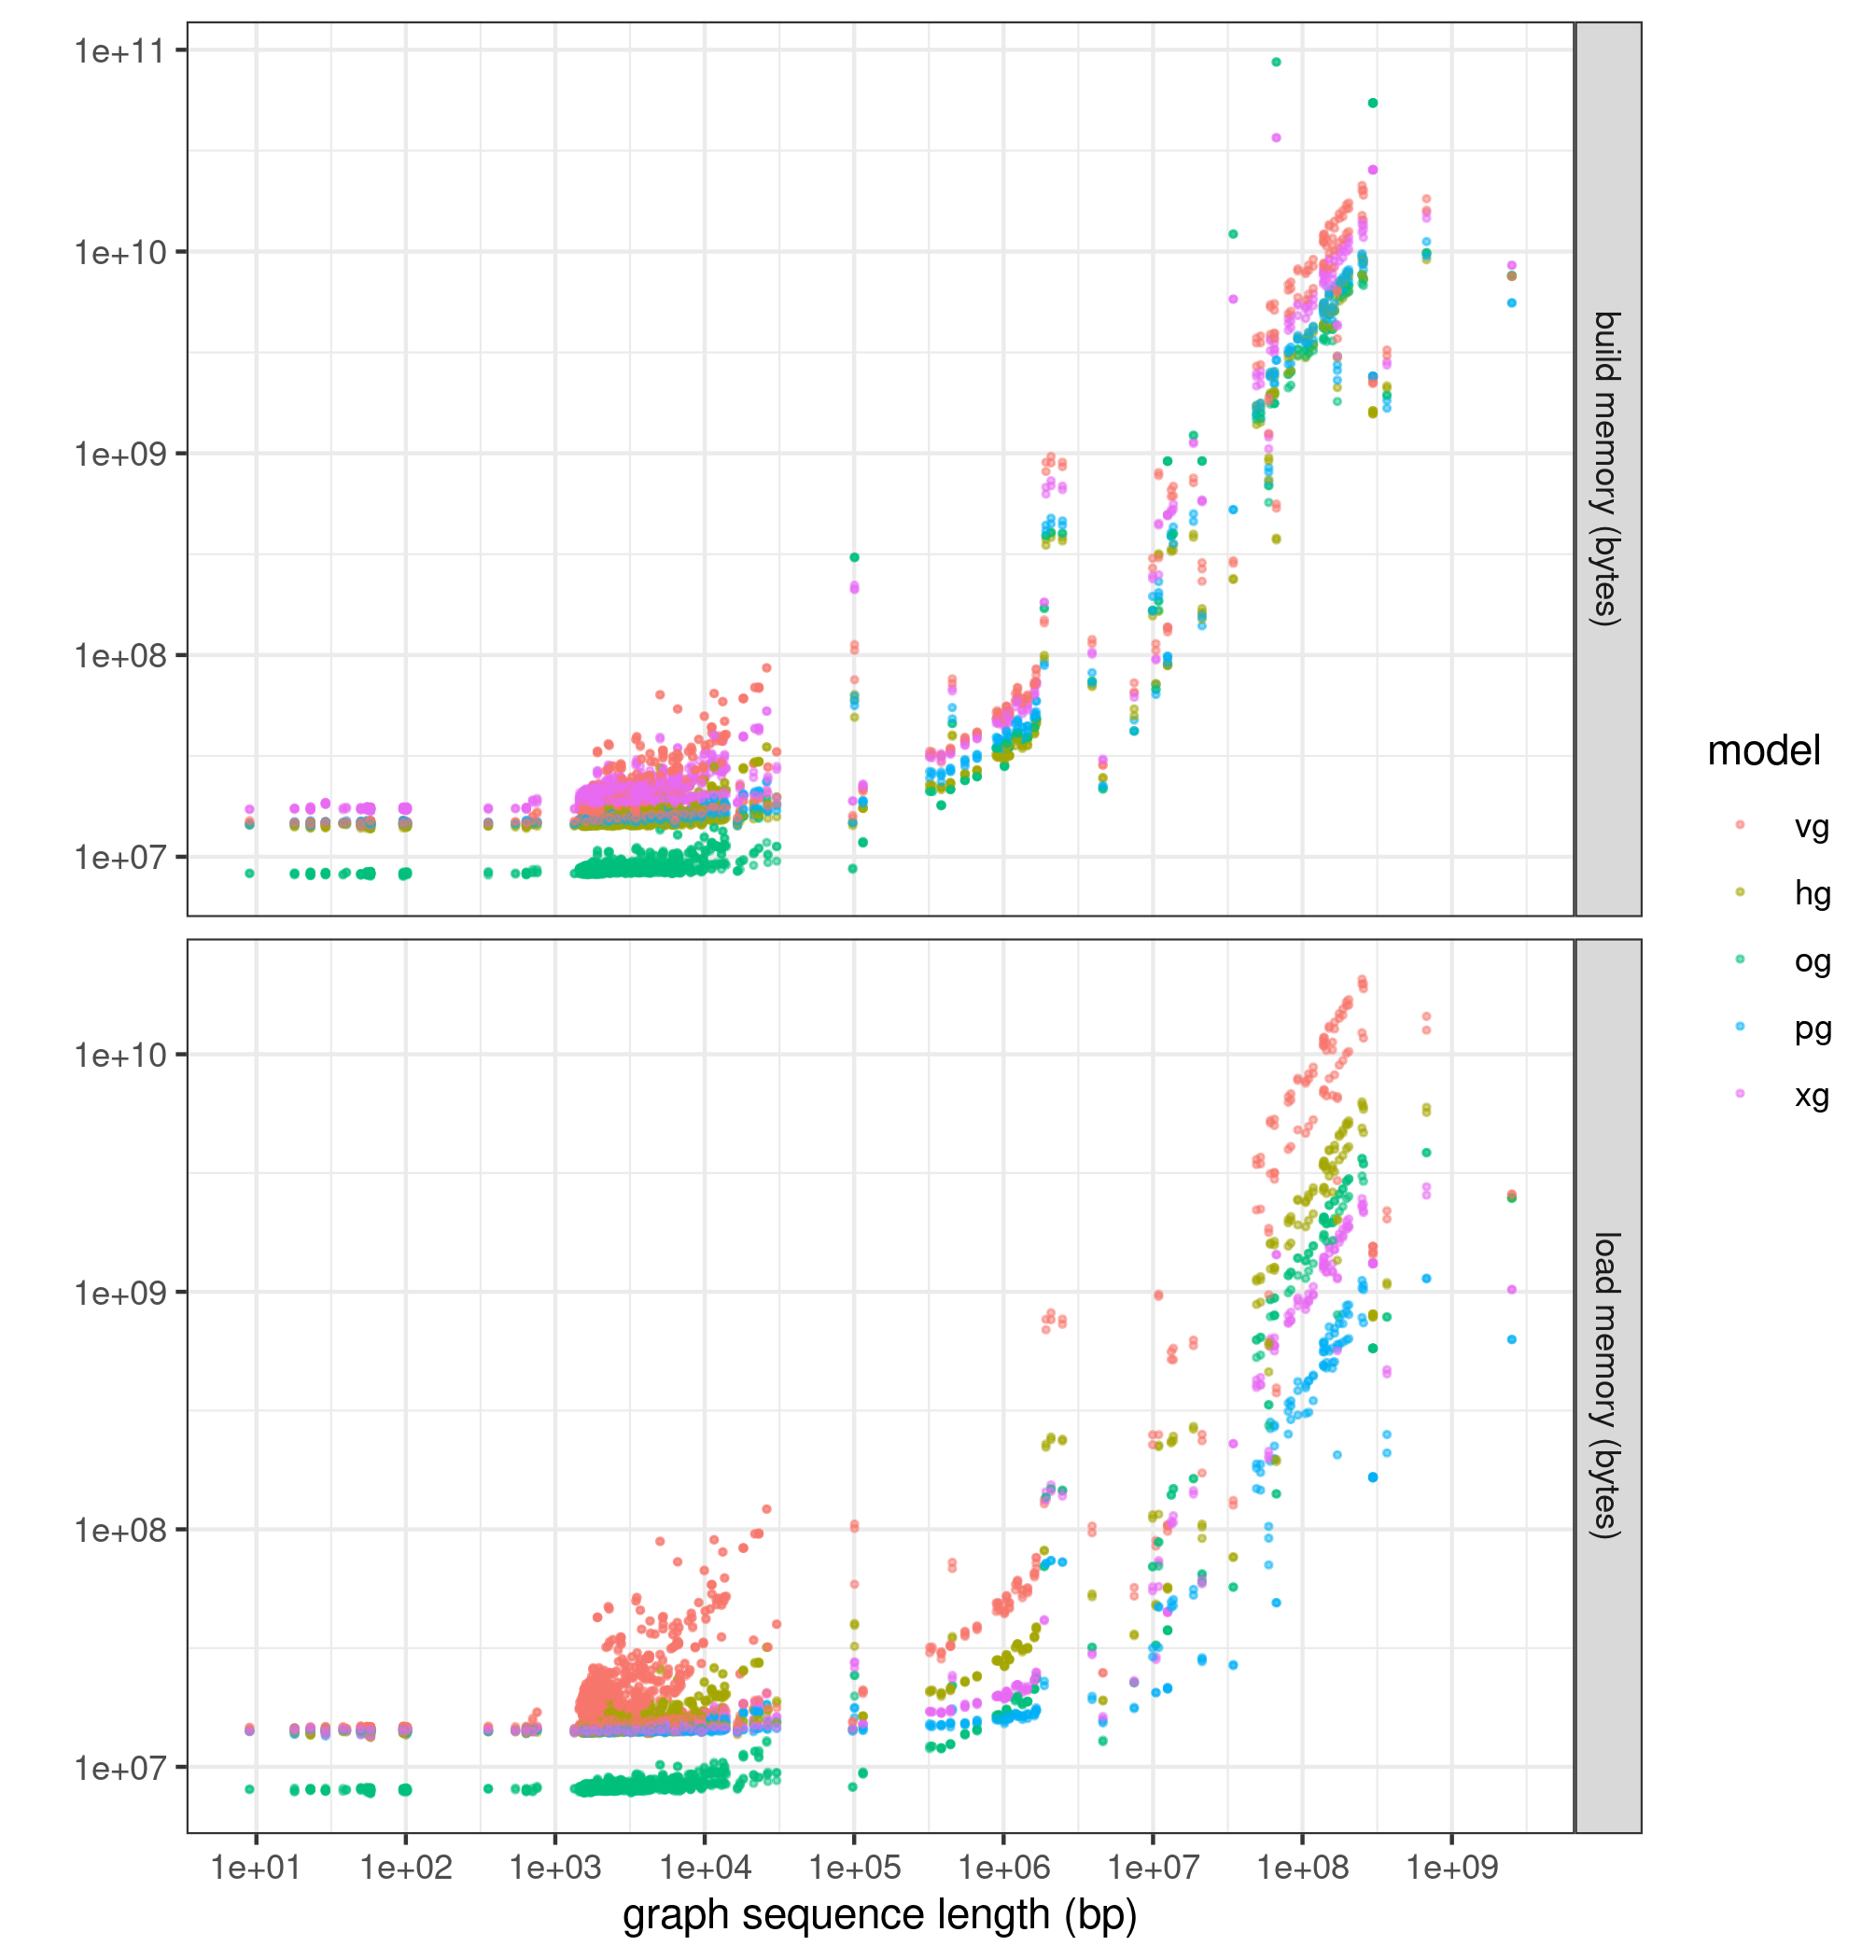
\includegraphics[width=0.5\textwidth]{figures/build_and_load_memory.png}
  \caption{
    \label{fig:prof1}
    \textbf{Memory requirements for model construction and loading.}
    Memory costs versus graph sequence size for the graph collection, colored by \textsc{HandleGraph} model.
    The memory requirements for graph construction tend to be higher than those for loading the graph model.
    All methods show fixed overheads of several megabytes, seen in the flat tail to the left of both plots.
    Outside of this region, all methods show roughly linear scaling in both build and load costs per input base pair.
    The relative differences in memory costs appear to be stable between different methods across many orders of magnitude in graph size.
    Notably, \textsc{vg} has approximately the same build and load costs, as the data structures used are the same.
    The other methods tend to use auxiliary data structures at build time, and so require more memory to build the data structure than to load it.
    }
\end{figure}

\begin{figure}
  \centering
  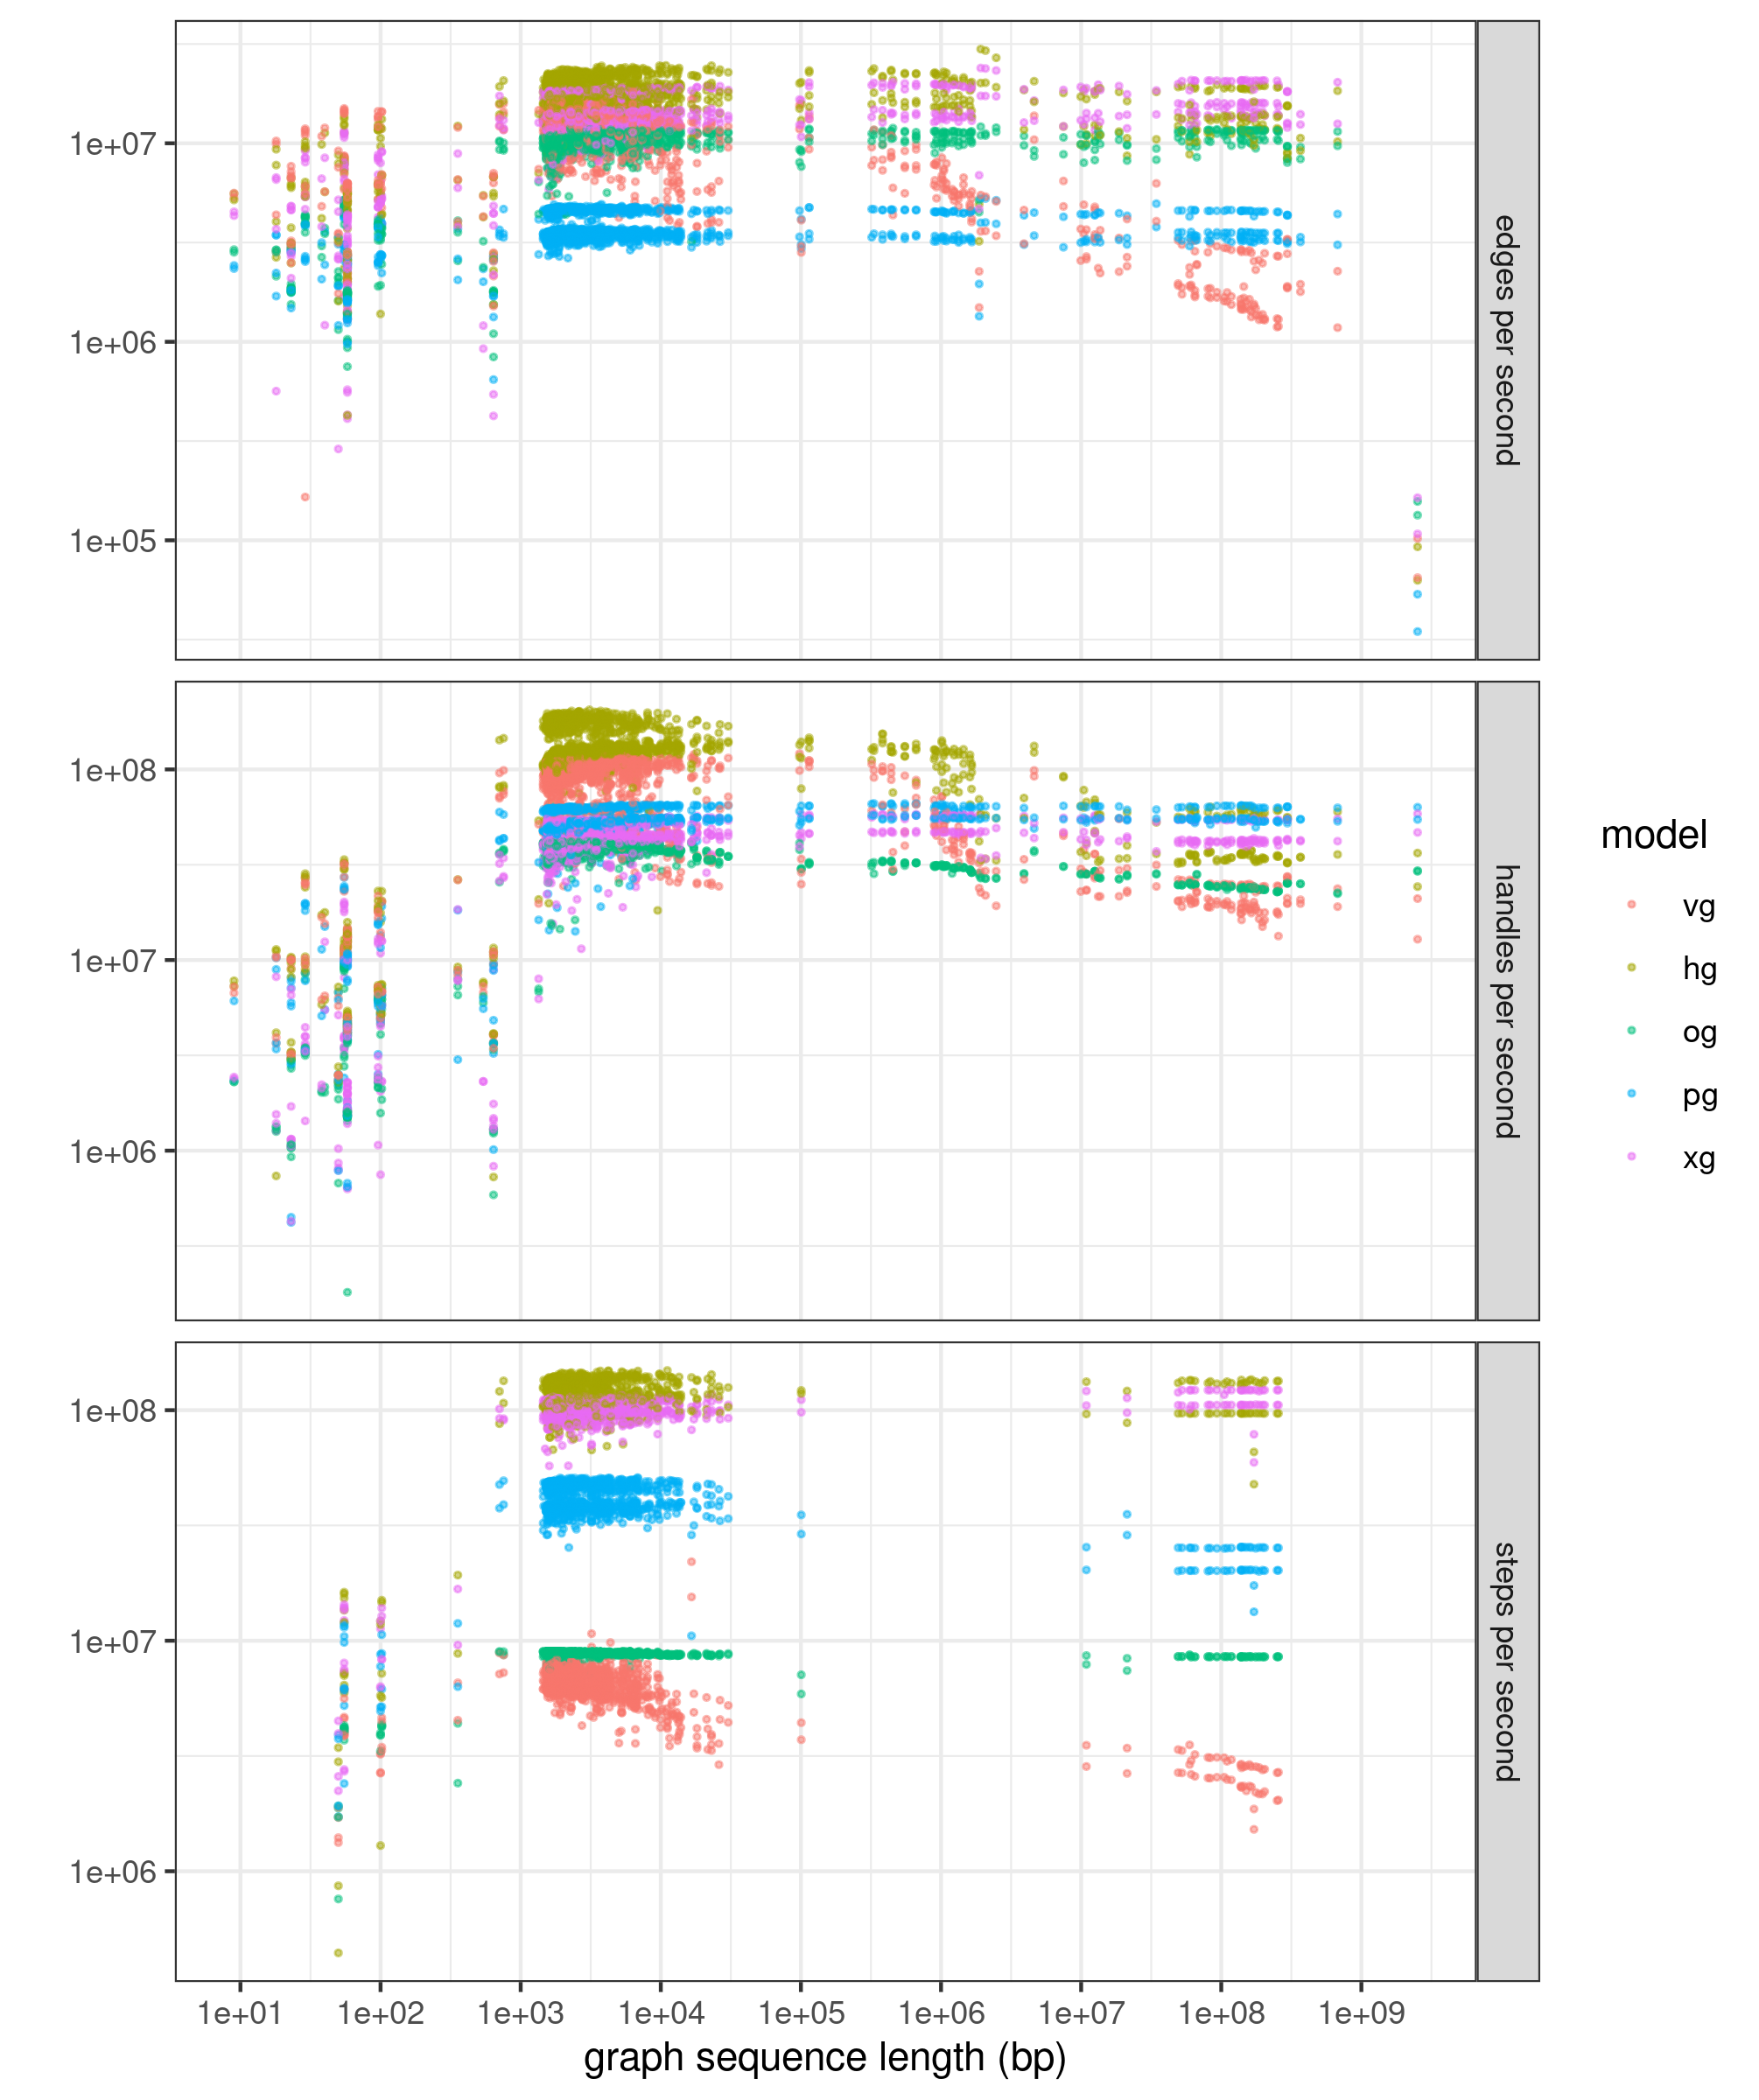
\includegraphics[width=0.5\textwidth]{figures/iteration_per_second.png}
  \caption{
    \label{fig:prof2}
    \textbf{Graph element enumeration performance.}
    Iteration performance for edges, nodes, and path steps for the full graph collection, shown in terms of elements per second.
    \textsc{HashGraph} provides the highest performance for all element iteration types on smaller graphs, but this performance falls of with larger graphs, presumably due to scaling properties of the backing hash tables.
    The same pattern can be seen for \textsc{vg}, although the overall performance is worse.
    Although it has the worst edge iteration performance, \textsc{PackedGraph} provides good performance on node and path step iteration.
    The relative path encoding in \textsc{odgi} yields poor performance on path iteration, and node decoding overheads appear to reduce its node iteration performance, but it has good graph topology traversal performance, perhaps due to cache efficiency of the edge encoding.
    \textsc{xg} provides excellent iteration performance in all cases.
    }
\end{figure}

To compare the methods' performances across a wide variety of different graphs, we applied each to a collection of 2299 graphs collected during our research on graphical pangenomics.
For each graph and graph implementation, we measured the same metrics described in the previous section as well as various graph properties including size, edge count, cyclicity, and path depth.
We summarize these results in Figures \ref{fig:prof1} and \ref{fig:prof2}.

For graph construction and loading, we observe similar trends as for the HGSVC graph.
\textsc{vg}'s performance in terms of memory usage is very poor, both during construction and load.
For construction and load, all models exhibit largely linear scaling characteristics, outside of very small graphs where static memory overheads dominate.
\textsc{PackedGraph} yields the best memory performance for larger graphs (which are mostly the chromosomes of the 1000 Genomes Project graph), while for the medium-sized graphs in the collection ($\sim$1~Mbp), \textsc{odgi} requires less memory.

For graph queries and iteration, the relative performance of the models is largely maintained across the entire range of graph sizes.
However, we observe that the hash-based models (\textsc{vg} and \textsc{HashGraph}) have very good performance for smaller graphs (in handle and edge enumeration) but decrease in throughput as the graph size increases.
Smaller, less dramatic decreases in performance can be seen for the other implementations.
For path enumeration, the highest-performing methods are \textsc{xg} and \textsc{HashGraph} at approximately 10 times faster than \textsc{odgi}, whose relative path storage is costly to traverse.

\subsection{1000 Genome Project chromosome graphs}

Variation graphs built from the 1000 Genomes Project (1000GP) variant catalog and the human reference genome have fairly homogenous and regular features.
In addition, they have connected components of very different sizes, each corresponding to a chromosome.
This provides a natural, fairly controlled means to explore the scaling behavior of our data structures.
Moreover, graphs of this form are seeing increasing use in variant-aware resequencing analyses \citep{crysnanto2019sequence}.
Thus, the performance of data structures on these graphs is of general interest.

\begin{figure}[p]
  \centering
  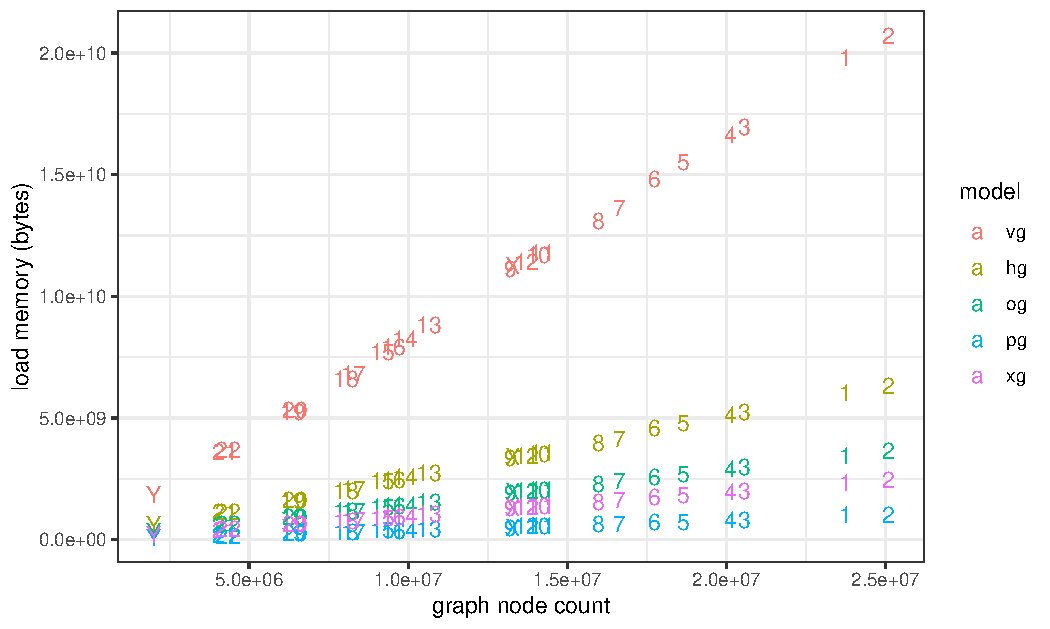
\includegraphics[width=0.5\textwidth]{figures/1000gp_chroms_node_count.pdf}
  \caption{
    \label{fig:1000GPchroms}
    \textbf{Load memory versus node count for chromosome graphs built from 1000 Genomes Project variants and GRCh37.}
    For each method, memory requirements are more strongly correlated with the number of nodes in the graph ($R^2 =$ 0.998) than with the graph sequence length ($R^2 =$ 0.986).
    Although the memory requirements are dominated by graph sequence size, node count will increase with variant density.
    Methods generally incur an overhead for each node that is larger than the sequence length.
    Linear scales clarify that the absolute difference in performance between \textsc{vg} and the other methods is significant.
    }
\end{figure}

We first evaluated the scaling performance of the various \textsc{HandleGraph} implementations relative to node count for each of the nuclear chromosomes in the 1000GP (Figure \ref{fig:1000GPchroms}).
We find that for all methods, load memory scales almost perfectly with node count, with an average $R^2 = 0.998$.
Due to differences in variant density among the chromosomes, the average correlation relative to sequence length is lower ($R^2 = 0.986$).

\begin{table}
  \centering
\begin{tabular}{c||c|c|r|r|r}
Model & Build B/bp & Load B/bp & $10^6$ Node/s & $10^6$ Edges/s & $10^6$ Steps/s \\
\hline
vg &   80.2 &                77.2  &              24.6 &                  2.8 &               2.9 \\
hg &   36.7 &                23.9  &              59.5 &                 18.9 &              \textbf{127.2} \\
og &   \textbf{30.3}  &   13.7  &              24.1 &                 11.5 &              8.2 \\
pg &   37.6 &                 \textbf{3.80}  &   \textbf{63.7} &   4.6 &                24.3 \\
xg &   54.3 &                9.31  &               54.2 &                 \textbf{20.5} & 117.0 \\
\hline
\end{tabular}
\caption{
  \textbf{Performance on 1000 Genomes Project chromosome graphs.}
  Average build memory, load memory, and iteration times for graph elements for the chromosome-level graphs built from all the variants in the 1000 Genomes Project and the GRCh37 reference genome against which the variant set was originally reported.
  \textsc{vg} requires $\sim$ 20 times as much memory to load the graphs as \textsc{PackedGraph}, while even the most costly \textsc{HandleGraph} model (\textsc{HashGraph}) requires $\sim$ 1/3 as much memory.
  In these graphs, \textsc{odgi} provides the lowest performance for handle iteration.
  However, in all other metrics, \textsc{vg} performs significantly worse than the other models.
}
\label{table:1000GPchroms}
\end{table}

In Table \ref{table:1000GPchroms}, we report the average memory performance of the methods relative to graph sequence length, and also the iteration performance in terms of elements per second.
We find that the best-performing method in terms of memory usage is \textsc{PackedGraph}, which consumes around $1/20$th the memory of \textsc{vg} per base-pair of graph in the 1000GP set.
However, it provides significantly better iteration performance for nodes (handles), edges, and path steps.
\textsc{HashGraph} and \textsc{xg} have similar iteration performance, but \textsc{xg}, by virtue of its use of compressed, static data structures, requires less than half as much memory.
\textsc{odgi} optimized for efficient dynamic operations on graphs with higher path coverage, and in general is not as performant as other methods on this set.


\section{Discussion}

We have presented a set of simple formalisms, the \textsc{HandleGraph} abstraction, which provides a coherent interface to address and manipulate the components of a genome variation graph.
To explore the utility of this model, we implemented data structures to encode variation graphs and matched them to this interface.
This allowed us to directly compare these \textsc{HandleGraph} implementations on a diverse set of genome graphs obtained during our research.
These experiments reveal that genome graphs need not pay the computational expense of the early versions of \textsc{vg}.
The best-performing models require an order of magnitude less memory than \textsc{vg} while providing higher performance for basic graph access operation and element iteration.
For these reasons, \textsc{vg} has transitioned to using these newer graph implementations. 

The efficiency of these methods and their encapsulation within a coherent programming interface will support their reuse within a diverse set of application domains.
Variation graphs have deep similarity with graphs used in assembly; these libraries could be used as the basis for assembly methods.
They could also be used for genotyping and haplotype inference methods based on graphs \citep{garg2018graph}.

Ongoing work is establishing large numbers of highly-contiguous whole genome assemblies for humans (\url{https://humanpangenome.org/}).
Improvements in sequencing technology are likely to make such surveys routine.
It is natural to consider a pangenome reference system, based on the whole genome alignments of such assemblies, as the output of these pangenome projects.
Recent results demonstrate that many basic bioinformatic problems can be generalized to operate on such structures.
Should these pangenome representations become common or standard, then variation graph data structures like those we have presented here will form the basis for a wide range of pangenomic methods.



%%%%%%%%%%%%%%%%%%%%%%%%%%%%%%%%%%%%%%%%%%%%%%%%%%%%%%%%%%%%%%%%%%%%%%%%%%%%%%%%%%%%%
%
%     please remove the " % " symbol from \centerline{\includegraphics{fig01.eps}}
%     as it may ignore the figures.
%
%%%%%%%%%%%%%%%%%%%%%%%%%%%%%%%%%%%%%%%%%%%%%%%%%%%%%%%%%%%%%%%%%%%%%%%%%%%%%%%%%%%%%%



%\section*{Acknowledgements}
%
%TODO

\section*{Funding}

This work was supported, in part, by the National Institutes of Health (award numbers U01HG010961, U41HG010972, R01HG010485, 2U41HG007234, 5U54HG007990, 5T32HG008345-04, U01HL137183 to B.P.) and the W. M. Keck Foundation (award number DT06172015 to B.P.).
S.H. acknowledges funding from the Central Innovation Programme (ZIM) for SMEs of the Federal Ministry for Economic Affairs and Energy of Germany.

\bibliographystyle{natbib}
%\bibliographystyle{achemnat}
%\bibliographystyle{plainnat}
%\bibliographystyle{abbrv}
%\bibliographystyle{bioinformatics}
%
%\bibliographystyle{plain}
%
\bibliography{document}


% \begin{thebibliography}{}

% \bibitem[Bofelli {\it et~al}., 2000]{Boffelli03}
% Bofelli,F., Name2, Name3 (2003) Article title, {\it Journal Name}, {\bf 199}, 133-154.

% \bibitem[Bag {\it et~al}., 2001]{Bag01}
% Bag,M., Name2, Name3 (2001) Article title, {\it Journal Name}, {\bf 99}, 33-54.

% \bibitem[Yoo \textit{et~al}., 2003]{Yoo03}
% Yoo,M.S. \textit{et~al}. (2003) Oxidative stress regulated genes
% in nigral dopaminergic neurnol cell: correlation with the known
% pathology in Parkinson's disease. \textit{Brain Res. Mol. Brain
% Res.}, \textbf{110}(Suppl. 1), 76--84.

% \bibitem[Lehmann, 1986]{Leh86}
% Lehmann,E.L. (1986) Chapter title. \textit{Book Title}. Vol.~1, 2nd edn. Springer-Verlag, New York.

% \bibitem[Crenshaw and Jones, 2003]{Cre03}
% Crenshaw, B.,III, and Jones, W.B.,Jr (2003) The future of clinical
% cancer management: one tumor, one chip. \textit{Bioinformatics},
% doi:10.1093/bioinformatics/btn000.

% \bibitem[Auhtor \textit{et~al}. (2000)]{Aut00}
% Auhtor,A.B. \textit{et~al}. (2000) Chapter title. In Smith, A.C.
% (ed.), \textit{Book Title}, 2nd edn. Publisher, Location, Vol. 1, pp.
% ???--???.

% \bibitem[Bardet, 1920]{Bar20}
% Bardet, G. (1920) Sur un syndrome d'obesite infantile avec
% polydactylie et retinite pigmentaire (contribution a l'etude des
% formes cliniques de l'obesite hypophysaire). PhD Thesis, name of
% institution, Paris, France.

% \end{thebibliography}
\end{document}
